%DLC development

\begin{frame}{KASCADE Cosmic-ray Data Center (KCDC)}
    \begin{itemize}
        \small
        \setlength{\itemsep}{0pt}
        \item providing free, unlimited, reliable open access to KASCADE cosmic ray data at \textcolor{blue}{\underline{https://kcdc.ikp.kit.edu}};
        \item almost all KASCADE data is available;
        \item selection of fully calibrated quantities and detector signals;
        \item information platform: physics and experiment backgrounds, tutorials, meta information for data analysis;
        \item archive of KASCADE software and data;
        \item uses modern and open source web technologies.
    \end{itemize}

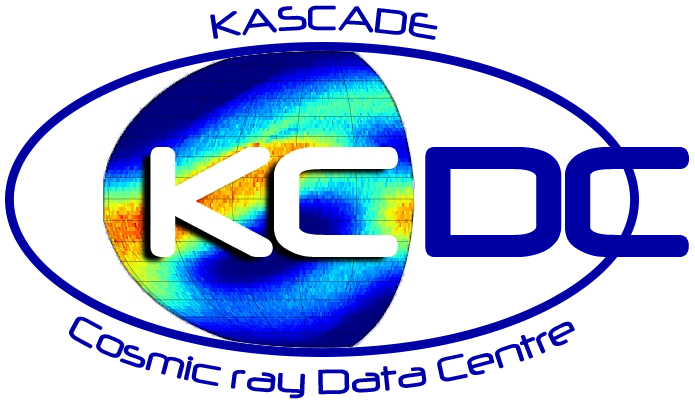
\includegraphics[height=0.35\textheight]{pics/KCDC-Logo.png}
\hfill
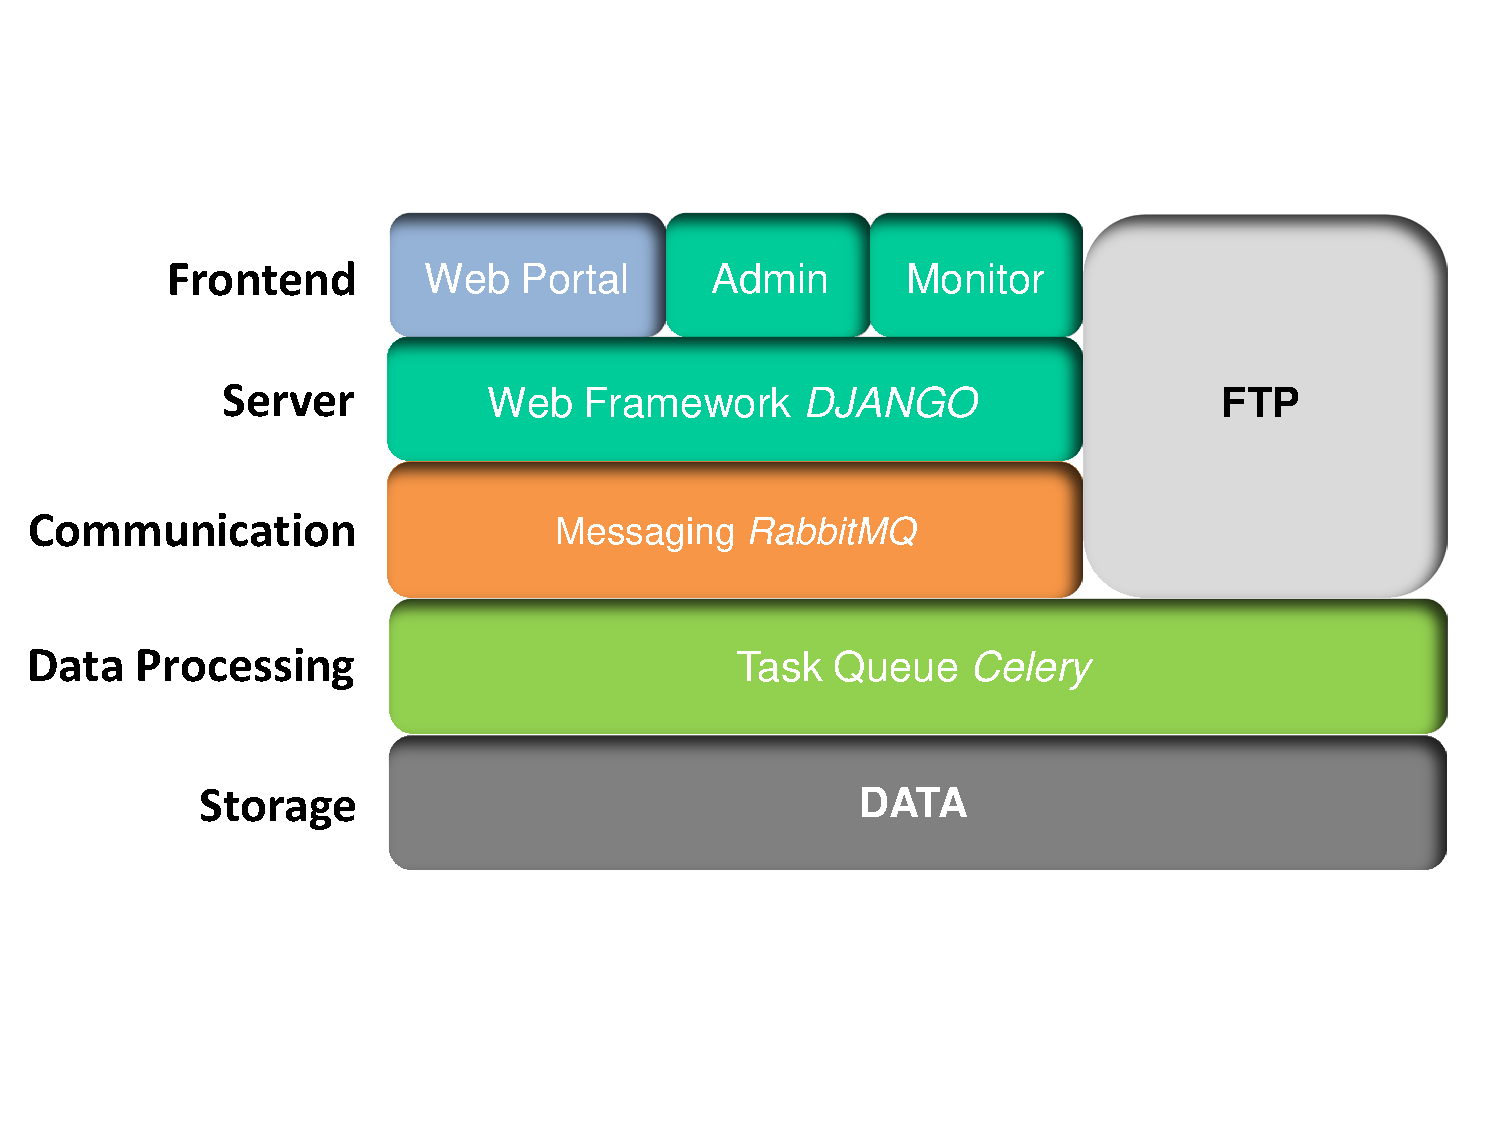
\includegraphics[height=0.35\textheight]{pics/KCDC-IT-Structure.pdf}
\end{frame}

\begin{frame}{KASCADE and TAIGA data rates}
\begin{minipage}[c]{0.5\textwidth}
  \begin{itemize}
    \item KASCADE:
    \begin{itemize}
      \item 450 000 000 events
      \item $\sim 4$~TB of measured data
    \end{itemize}
    \vspace{2em}
    \item planned TAIGA rate: $\sim 20$~TB/year
    \begin{itemize}
      \item HiSCORE: $\sim 18$~TB/year
      \item IACT: $\sim 1.5$~TB/year
      \item others: $\sim 0.5$~TB/year
    \end{itemize}
  \end{itemize}
\end{minipage}
\hfill
\begin{minipage}[c]{0.49\textwidth}
\vspace{-3.5em}
  \begin{itemize}
    \item current TAIGA rate: 
    \begin{itemize}
      \item $\sim 50$~TB of raw data;
      \item $\sim 8$~TB/year of reconstructed data:
      \begin{itemize}
        \item HiSCORE: $\sim 6.4$~TB/year
        \item IACT: $\sim 1$~TB/year
        \item others: $\sim 0.5$~TB/year
      \end{itemize}
    \end{itemize}
  \end{itemize}
\end{minipage}
\end{frame}
% 
\begin{frame}{DLC Architecture}
\begin{center}
  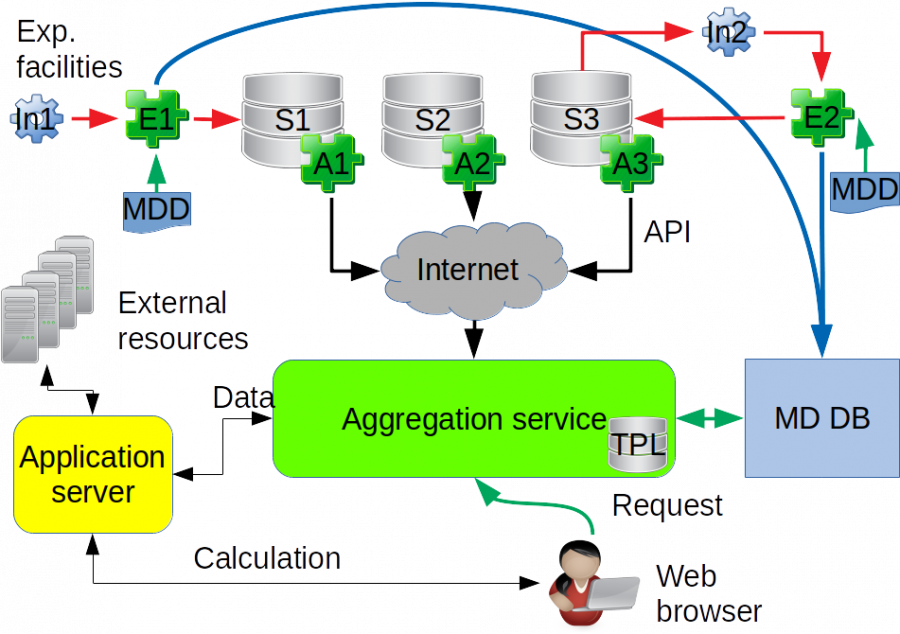
\includegraphics[width=0.8\textwidth]{pics/arch_appds.png}
\end{center}
\end{frame}
